\chapter{函数性质}
函数能够很好的描述一样东西的变化规律,从而得出结论(从先前章节的笔记就可以看出)。但这还不够,想要深入分析,我们还是要了解更多的知识。

在本章中,你会学习一些新的函数及其图像。再依靠图像,得出函数的某些性质,并证明之。

\section{函数图像}
在初中我们学过一次函数、反比例函数以及二次函数,它们的图像就不再介绍了。如记性不好的请请教初中数学老师。

顺带提一句:下文讲述的函数的绘制方法只能画出近似的、粗略的函数图像,这种精度在绝大多数情况下是没有问题的\footnote{例外情况指方程的解的个数问题,前文已经提过。},您也应该在绝大多数情况下绘制这种图像。

对于三角函数,会在后面的“三角函数”章节提到。这里仅仅画出它们的图像而不研究其性质。

\subsection{耐克函数}
首先介绍的是耐克函数(或称对勾函数),它的解析式形如:\[y=ax+\frac{b}{x}\]

通过描点法,不难画出它的图像(如图\ref{fig:figure-of-tick-functions})。

\begin{figure}[htb]
	\centering
	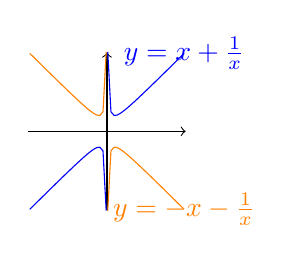
\begin{tikzpicture}[scale=0.1]
		\draw[->] (-10, 0) -- (10, 0);
		\draw[->] (0, -10) -- (0, 10);
		\draw[color=blue, domain=0.1:9.8] plot(\x, \x + 1 / \x) node {$y=x+\frac{1}{x}$};
		\draw[color=blue, domain=-9.8:-0.1] plot(\x, \x + 1 / \x);
		\draw[color=orange, domain=0.1:9.8] plot(\x, -\x - 1 / \x) node {$y=-x-\frac{1}{x}$};
		\draw[color=orange, domain=-9.8:-0.1] plot(\x, -\x - 1 / \x);
	\end{tikzpicture}
	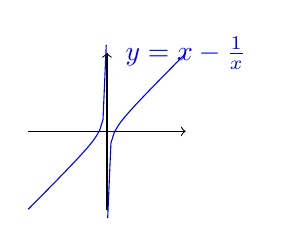
\begin{tikzpicture}[scale=0.1]
		\draw[->] (-10, 0) -- (10, 0);
		\draw[->] (0, -10) -- (0, 10);
		\draw[color=blue, domain=0.09:10] plot(\x, \x - 1 / \x) node {$y=x-\frac{1}{x}$};
		\draw[color=blue, domain=-10:-0.09] plot(\x, \x - 1 / \x);
	\end{tikzpicture}
	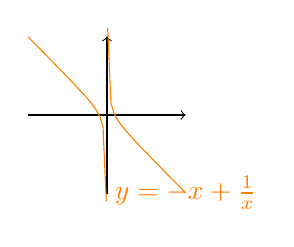
\begin{tikzpicture}[scale=0.1]
		\draw[->] (-10, 0) -- (10, 0);
		\draw[->] (0, -10) -- (0, 10);
		\draw[color=orange, domain=0.09:10] plot(\x, -\x + 1 / \x) node {$y=-x+\frac{1}{x}$};
		\draw[color=orange, domain=-10:-0.09] plot(\x, -\x + 1 / \x);
	\end{tikzpicture}
	\caption{参量取不同值时耐克函数的图像}
	\label{fig:figure-of-tick-functions}
\end{figure}

然后我们可以得出耐克函数的性质:

\begin{itemlist}
	\item $a^+,b^+$是一、三象限的耐克函数
	\item $a^-,b^-$是二、四象限的耐克函数
	\item $a^-,b^+$是双增函数
	\item $a^+,b^-$是双减函数
\end{itemlist}

再看一眼函数图像,$a$、$b$同号时在各个象限内有极值点,接下来将推导出这个点的坐标:

\begin{quote}
	根据基本不等式得:\[ax+\frac{b}{x}\geq2\sqrt{ab}\]

	此时不等号右边即极值点的纵坐标,代入原式解方程:
	\[\begin{split}
		&ax+\frac{b}{x}=2\sqrt{ab} \\
		&ax^2-2x\sqrt{ab}+b=0 \\
		&x=\sqrt{\frac{b}{a}}
	\end{split}\]

	可以得到耐克函数在第一象限内的顶点坐标为$(\sqrt{\frac{b}{a}},2\sqrt{ab})$,其它象限只需在对应的地方添负号即可。
\end{quote}

\subsection{幂函数}
在初中我们学过了反比例函数、二次函数,它们都是幂函数的一种。其解析式为:\[y=x^a\]其中$a=\frac{p}{q}$,$p,q\in\mathbb{Z}$。

要绘制幂函数的图像,应把第一象限的图像和其余部分的图像分别绘制。

第一象限的图像如图\ref{fig:figure-of-power-function}所示。

\begin{figure}[htb]
	\centering
	\begin{subfigure}[b]{0.3\textwidth}
		\centering
		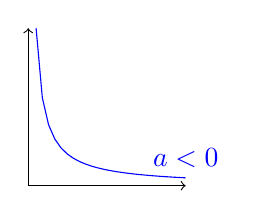
\begin{tikzpicture}[scale=0.2]
			\draw[->] (0, 0) -- (10, 0);
			\draw[->] (0, 0) -- (0, 10);
			\draw[color=blue, domain=0.5:10] plot(\x, 5 / \x) node[above] {$a<0$};
		\end{tikzpicture}
		\caption{减}
	\end{subfigure}
	\begin{subfigure}[b]{0.3\textwidth}
		\centering
		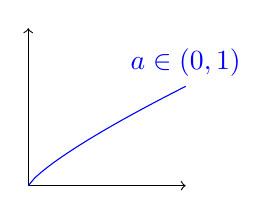
\begin{tikzpicture}[scale=0.2]
			\draw[->] (0, 0) -- (10, 0);
			\draw[->] (0, 0) -- (0, 10);
			\draw[color=blue, domain=0:10] plot(\x, \x ^ 0.8) node[above] {$a\in(0,1)$};
		\end{tikzpicture}
		\caption{缓慢增}
	\end{subfigure}
	\begin{subfigure}[b]{0.3\textwidth}
		\centering
		\begin{tikzpicture}[scale=0.2]
			\draw[->] (0, 0) -- (10, 0);
			\draw[->] (0, 0) -- (0, 10);
			\draw[color=blue, domain=0:6.81] plot(\x, \x ^ 1.2) node[right] {$a>1$};
		\end{tikzpicture}
		\caption{快速增}
	\end{subfigure}
	\caption{幂函数第一象限内的图像}
	\label{fig:figure-of-power-function}
\end{figure}

其它象限的图像可按照下面的流程绘出:
\[\begin{cases}
	\text{$q$为偶数} & \text{只有第一象限图像} \\
	\text{$q$为奇数} & \text{判断$p$}
	\begin{cases}
		\text{$p$为奇数} & \text{函数为奇函数} \\
		\text{$p$为偶数} & \text{函数为偶函数}
	\end{cases}
\end{cases}\]

\section{反函数}
我们知道,将某一个特定的值代入函数的自变量(即$x$)可以求出因变量(即$y$)的值。那已知$y$求$x$呢?解方程即可。

那我们就可以更进一步,直接用$y$来表示$x$,那就是\textbf{反函数}了。

由于函数需要$x$对应一个$y$,所以我们可以得到$x$、$y$\textbf{一一对应}是反函数存在的充要条件。

\section{导数}
在之前的笔记中,单调性可以描述一个函数在某一区间的增减性。但它具有局限性:我们只能知道一个大体的情况(增、减或非单调),而不能知道它的具体增减量为何。

再设想一下:我们通过描点法画出了函数上的几个点,要使用曲线连接把它们连接起来。由于两点之间的距离比较大,我们可能会画出几种不同的图像(如图\ref{fig:two-different-function-figure})。

\begin{figure}[htb]
    \centering
    \begin{tikzpicture}
        \draw[->] (-2, 0) -- (2, 0);
        \draw[->] (0, -2) -- (0, 2);
        \filldraw (-1, 0.5) circle [radius=1pt] (0, 1.2) circle [radius=1pt] (1, 0.8) circle [radius=1pt];
        \draw[color=blue,domain=-2:2] plot (\x, -0.55*\x*\x+0.15*\x+1.2);
        \draw[color=red,domain=-1.2:-0.8] plot (\x, -0.55*\x*\x+0.15*\x+1.2);
    \end{tikzpicture}
    \begin{tikzpicture}
        \draw[->] (-2, 0) -- (2, 0);
        \draw[->] (0, -2) -- (0, 2);
        \filldraw (-1, 0.5) circle [radius=1pt] (0, 1.2) circle [radius=1pt] (1, 0.8) circle [radius=1pt];
        \draw[color=orange,domain=-1.26346:1.2423] plot (\x, 2.1667*\x*\x*\x-0.55*\x*\x-2.01667*\x+1.2);
    \end{tikzpicture}
    \caption{描点法作出的两种截然不同的图像}
    \label{fig:two-different-function-figure}
\end{figure}

当然,我们可以描更多的点作更精确的图像,那可就无穷无尽了。

不过如果我们知道最左边描的一点附近的斜率比较小,那我们可以知道左图描红的部分绘制地更精确一些。

综上可以看出:过去研究的函数及其性质存在不足。故需要引入新的东西,叫做\textbf{导数}\footnote{“导数”即导函数,函数某一点处的斜率称为“导数值”。}。

求函数某一点导数值的公式如下\footnote{极限的求法不是重点,故不介绍。所以请自己领悟(笑)}:\[f'(x_0)=\lim_{h\rightarrow 0}\frac{f(x_0+h)-f(x_0)}{h}\]其几何意义是$y=f(x)$在点$P(x_0, f(x_0))$处切线的斜率。

\begin{quote}
	使用计算器的$\frac{d}{dx}$功能,可以直接求出导数值(需要处于“计算”模式下)。
\end{quote}

知道了函数某一点处的斜率,我们就可以根据下面的公式:\[y-f(x_0)=f'(x_0)(x-x_0)\]求出该点的切线方程。

\begin{example}
	利用导数的定义求$y=x^2$在$x=1$处的导数$f'(1)$,并求此函数在$x=1$时的切线方程

	\begin{quote}
		先套公式得导数值:\[f'(1)=\lim_{h\rightarrow 0}\frac{(1+h)^2-1}{h}=\lim_{h\rightarrow 0}h+2=2\]
		然后求得切线方程:\[y-1=2(x-1)\Rightarrow y=2x-1\]
	\end{quote}
\end{example}

将求导数值的公式稍作修改,就可以得到导函数的定义求法:\[f'(x)=\lim_{h\rightarrow 0}\frac{f(x+h)-f(x)}{h}\]

\begin{example}
	用定义求$f(x)=x^2$的导函数

	\begin{quote}
		这道例题很简单,只需带入公式即可:\[f'(x)=\lim_{h\rightarrow 0}\frac{(x+h)^2-x^2}{h}=\lim_{h\rightarrow 0}2x+h=2x\]
	\end{quote}
\end{example}

\subsection{求导函数}
在上文,我们求出了$y=x^2$的导函数。使用定义求法当然可以求出很多函数的导函数。不过由于知识水平有限,更多函数的导函数是算不出来的,所以下面这个列表整理了基础函数的导函数:

\begin{desclist}
	\item[多项式函数] $(C)'=0$;$(x^a)'=ax^{a-1}$
	\item[指对函数] $(e^x)'=e^x$;$(\ln x)'=\frac{1}{x}$
	\item[三角函数] $(\sin x)'=\cos x$;$(\cos x)'=-\sin x$
\end{desclist}

我们知道初等数学中代数式有四则运算,那导数呢?肯定有四则运算,它的运算法则如下:

\begin{desclist}
	\item[加减法] $(f\pm g)'=f'\pm g'$
	\item[数乘] $(Cf)'=C\cdot f'$
	\item[乘法] $(f\cdot g)'=f'g+fg'$
	\item[除法] $(\frac{f}{g})'=\frac{f'g-fg'}{g^2}$
\end{desclist}

\begin{quote}
	如果不按照运算法则去计算导数,而仅仅凭错误的经验,老师说不定会生气到想要揍你哦(苦笑)
\end{quote}

咳咳,回到正题。注意四则运算中没有包括指数运算,不过这个是小事情,不用担心,过一会儿会介绍指数函数的求导。

\noindent\dotfill

要求对数函数的导数,要先利用换底公式:$\log_ax=\frac{\ln x}{\ln a}$,然后使用指对函数的求导公式求导:
\[(\log_ax)'=\frac{1}{x\ln a}\]

\begin{example}
	求$y=\log_2x$的导数

	\begin{quote}
		\[\begin{aligned}
			y'&=(\log_2x)'=(\frac{\ln x}{\ln2})' \\
			  &=(\frac{1}{\ln2}\cdot\ln x)'=\frac{1}{x\ln2}
		\end{aligned}\]
		注意$\frac{1}{\ln2}$是一个常数,可以提出。
	\end{quote}
\end{example}

\noindent\dotfill

求三角函数的导数,需要全部化到一倍角后利用切割化弦,全部换成$\sin$和$\cos$后利用三角函数的求导公式求导。

其它三角函数的导函数:

\[
	\begin{aligned}
		(\tan x)'&=\sec^2x \\
		(\cot x)'&=-\csc^2x \\
		(\sec x)'&=\tan x\cdot\sec x \\
		(\csc x)'&=-\cot x\cdot\csc x \\
	\end{aligned}
\]

\subsubsection{复合函数的导数}
刚刚我们求过了$y=\sin2x$的导函数,这明显太麻烦了。
